% ============================================================================
% Presentación oral — Trabajo Práctico Final de Deep Learning
% Sistema de Detección y Segmentación de Objetos en Tiempo Real
% Autor: Federico Morán
% Compilar: pdflatex presentacion.tex  (dos pasadas)
% ============================================================================
\documentclass[aspectratio=169,11pt]{beamer}

\usepackage[utf8]{inputenc}
\usepackage[T1]{fontenc}
\usepackage{lmodern}
\usepackage[spanish,es-tabla,es-noquoting]{babel}
\usepackage{graphicx}
\usepackage{booktabs}
\usepackage{amsmath}
\usepackage{xcolor}
\usepackage{tikz}
\usetikzlibrary{arrows.meta,positioning,shapes.geometric}

\usetheme{Boadilla}
\setbeamertemplate{navigation symbols}{}
\setbeamertemplate{caption}[numbered]
\setbeamercovered{transparent}

% --- Paleta coherente con las figuras del informe -----------------------------
\definecolor{azul}{HTML}{2A78D6}
\definecolor{aqua}{HTML}{1BAF7A}
\definecolor{ambar}{HTML}{EDA100}
\definecolor{rojo}{HTML}{E34948}
\definecolor{gris}{HTML}{5A5A5A}

\setbeamercolor{structure}{fg=azul}
\setbeamercolor{title}{fg=white,bg=azul}
\setbeamercolor{frametitle}{fg=white,bg=azul}
\setbeamercolor{block title}{fg=white,bg=azul}
\setbeamercolor{block title alerted}{fg=white,bg=rojo}
\setbeamercolor{block title example}{fg=white,bg=aqua}
\setbeamerfont{frametitle}{size=\large}
\setbeamerfont{title}{series=\bfseries}

\usepackage{listings}

% --- Estilo de los listados (coherente con el informe) -----------------------
\definecolor{codebg}{RGB}{247,248,250}
\definecolor{coderule}{RGB}{223,226,230}
\definecolor{codekw}{RGB}{0,72,153}
\definecolor{codestr}{RGB}{163,21,21}
\definecolor{codecom}{RGB}{106,115,125}

\lstdefinestyle{py}{
  language=Python,
  basicstyle=\ttfamily\scriptsize,
  keywordstyle=\color{codekw}\bfseries,
  stringstyle=\color{codestr},
  commentstyle=\color{codecom}\itshape,
  backgroundcolor=\color{codebg},
  frame=single, framesep=4pt, rulecolor=\color{coderule},
  breaklines=true, showstringspaces=false, tabsize=2,
  columns=fullflexible, keepspaces=true,
  extendedchars=true, upquote=true,
  aboveskip=0.6em, belowskip=0.4em,
  literate={á}{{\'a}}1 {é}{{\'e}}1 {í}{{\'i}}1 {ó}{{\'o}}1 {ú}{{\'u}}1 {ñ}{{\~n}}1,
}

\graphicspath{{../reporte/figuras/}}

% Marcador de contenido pendiente (se elimina al cerrar los resultados)
\newcommand{\pend}[1]{\textcolor{rojo}{\textbf{[PENDIENTE: #1]}}}

% Pie de página compacto
\setbeamertemplate{footline}{%
  \hbox{%
    \begin{beamercolorbox}[wd=.5\paperwidth,ht=2.4ex,dp=1ex,leftskip=1em]{author in head/foot}%
      \usebeamerfont{author in head/foot}\insertshortauthor
    \end{beamercolorbox}%
    \begin{beamercolorbox}[wd=.5\paperwidth,ht=2.4ex,dp=1ex,rightskip=1em]{author in head/foot}%
      \hfill\insertframenumber{} / \inserttotalframenumber
    \end{beamercolorbox}}%
  \vskip0pt%
}

\title[Detección y segmentación en tiempo real]{Sistema de Detección y Segmentación de
Objetos en Tiempo Real mediante Ajuste Fino de YOLOv8}
\subtitle{Trabajo Práctico Final --- Deep Learning}
\author[Federico Morán]{Federico Morán}
\institute[Maestría en IA]{Maestría en Inteligencia Artificial}
\date{Julio de 2026}

\begin{document}

% ============================================================================
\begin{frame}[plain]
  \titlepage
\end{frame}

% ============================================================================
\begin{frame}{Contenidos}
  \tableofcontents
\end{frame}

% ============================================================================
\section{Problema y objetivo}

\begin{frame}{Problema y objetivo}
  \begin{block}{Objetivo general}
    Desarrollar un sistema completo de visión por computadora que \textbf{detecte y
    segmente objetos en tiempo real} sobre hardware de consumo.
  \end{block}

  \vspace{0.6em}
  \textbf{Objetivos específicos}
  \begin{enumerate}
    \item Construir un conjunto de datos supervisado a partir de COCO 2017.
    \item Ajustar un modelo de segmentación de instancias por transferencia de aprendizaje.
    \item Evaluarlo con las métricas estándar del área (mAP e IoU, cajas y máscaras),
          incluida la comparación contra el modelo preentrenado de referencia.
    \item Implementar la inferencia en tiempo real con captura de cámara web.
  \end{enumerate}

  \vspace{0.6em}
  \begin{alertblock}{¿Por qué importa el tiempo real?}
    Robótica, asistencia, control de inventario y análisis de video imponen un compromiso
    exigente entre \textbf{precisión} y \textbf{latencia}, en particular sin aceleración
    dedicada.
  \end{alertblock}
\end{frame}

\begin{frame}{Detección y segmentación: dos tareas, un modelo}
  \begin{columns}[T]
    \begin{column}{0.48\textwidth}
      \textbf{Detección}\\[0.3em]
      Localiza cada objeto con una \emph{caja delimitadora} y le asigna una clase.
      \vspace{1em}

      \textbf{Segmentación de instancias}\\[0.3em]
      Delimita, \emph{píxel a píxel}, la silueta exacta de cada objeto individual.
      \vspace{1em}

      \begin{exampleblock}{Clave}
        YOLOv8-seg resuelve \textbf{ambas} tareas con una única pasada hacia adelante:
        la cabeza predice caja, clase y coeficientes de máscara simultáneamente.
      \end{exampleblock}
    \end{column}
    \begin{column}{0.48\textwidth}
      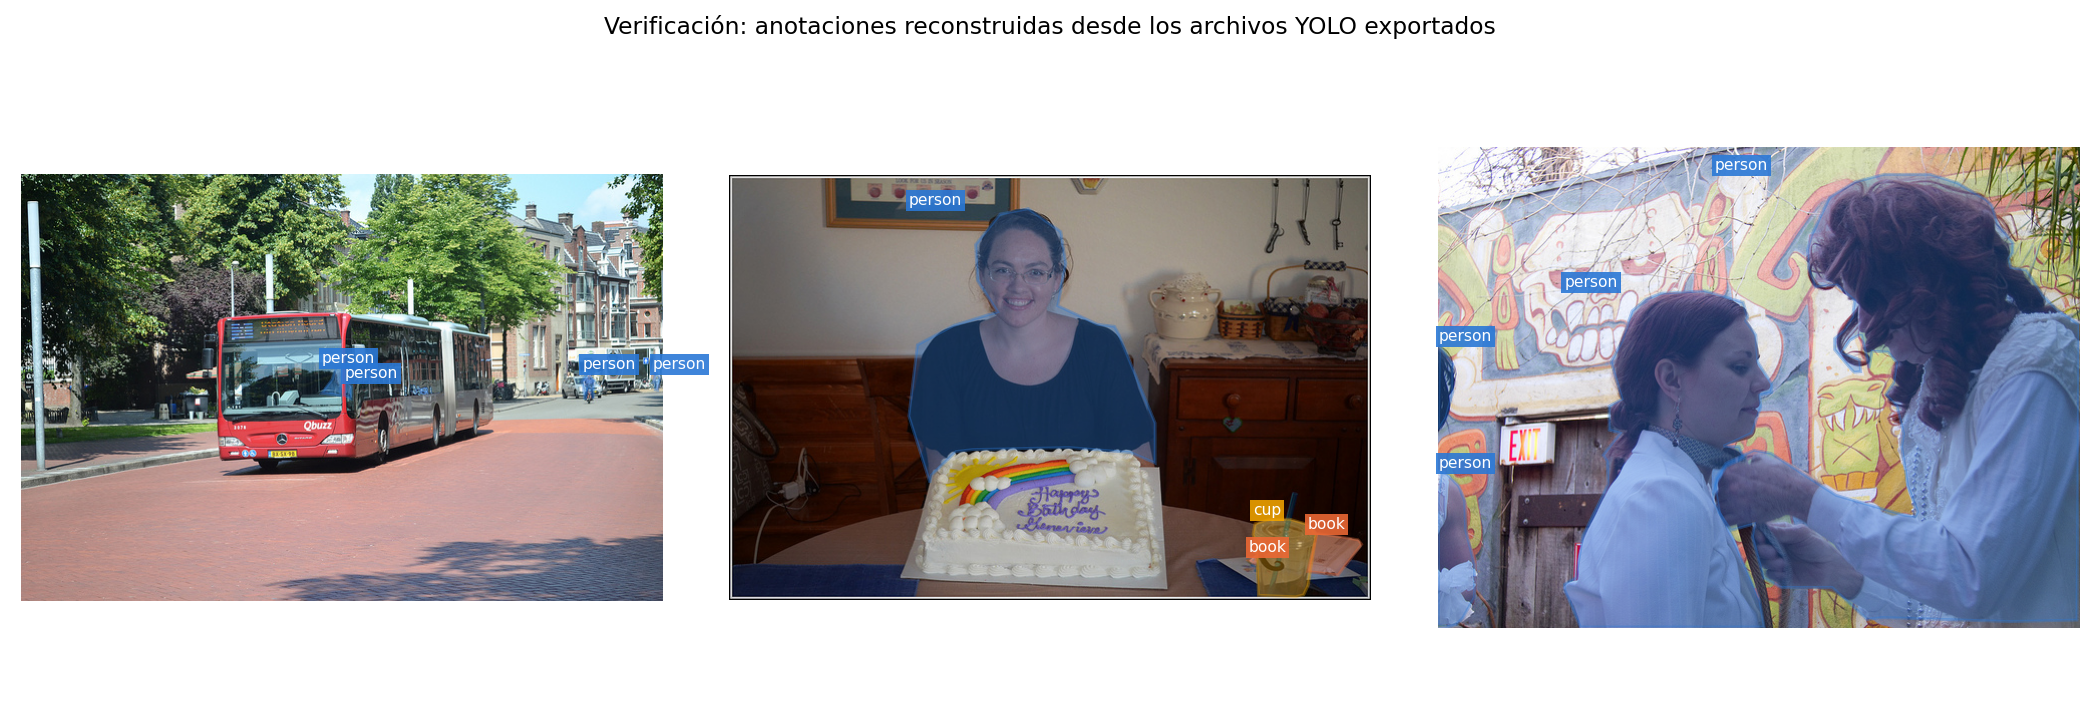
\includegraphics[width=\textwidth]{verificacion_etiquetas.png}
      \\[0.3em]
      {\scriptsize Anotaciones de instancia reconstruidas desde los archivos YOLO
      exportados: cada objeto tiene caja \emph{y} polígono.}
    \end{column}
  \end{columns}
\end{frame}

\begin{frame}{Alcance: ocho clases de entorno doméstico y de oficina}
  \begin{columns}[T]
    \begin{column}{0.5\textwidth}
      \texttt{person} \quad \texttt{cell phone} \quad \texttt{cup}\\
      \texttt{bottle} \quad \texttt{laptop} \quad \texttt{keyboard}\\
      \texttt{mouse} \quad \texttt{book}
      \vspace{1em}

      \textbf{Criterio de selección}\\[0.3em]
      Todas pueden \textbf{exhibirse físicamente} ante una cámara web durante la
      demostración en vivo. El criterio es de aplicación, no de conveniencia estadística.
      \vspace{1em}

      Los objetos de las restantes 72 categorías de COCO pasan a formar parte del
      \textbf{fondo}, lo que define con precisión el alcance del problema.
    \end{column}
    \begin{column}{0.5\textwidth}
      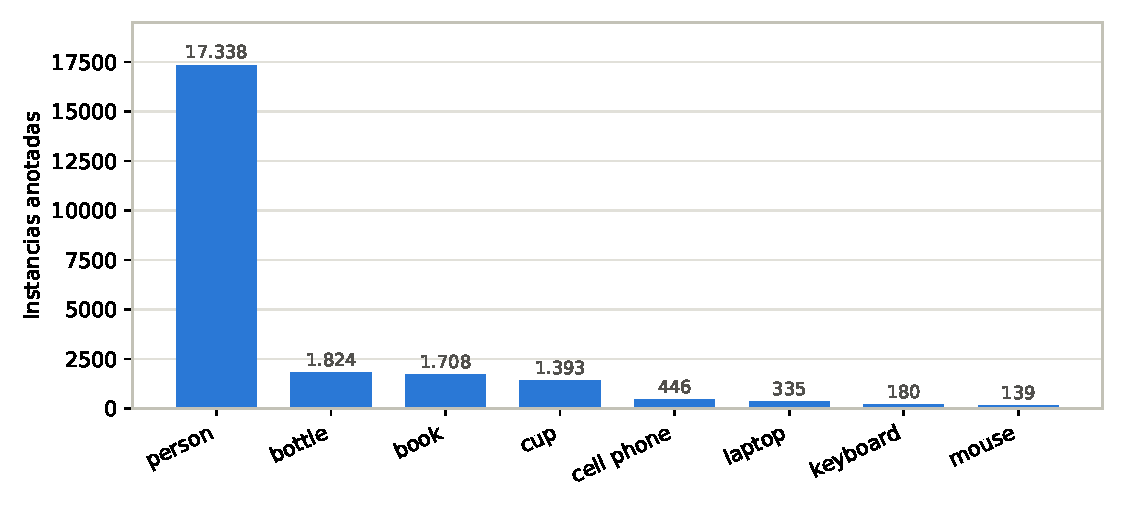
\includegraphics[width=\textwidth]{dist_clases.pdf}
      \\[0.3em]
      {\scriptsize Desbalance pronunciado, heredado de la estadística natural de COCO:
      \texttt{person} concentra el 74,2\,\% de las instancias; \texttt{mouse} reúne 139.}
    \end{column}
  \end{columns}
\end{frame}

% ============================================================================
\section{Datos y metodología}

\begin{frame}{Pipeline de extremo a extremo}
  \centering
  \begin{tikzpicture}[
      node distance=0.42cm and 0.5cm,
      caja/.style={rectangle, rounded corners=2pt, draw=azul!70, fill=azul!8,
                   text width=2.3cm, align=center, font=\scriptsize, minimum height=1.15cm},
      cajav/.style={caja, draw=aqua!80, fill=aqua!10},
      flecha/.style={-{Stealth[length=2mm]}, draw=gris, thick}]

    \node[caja] (a) {Descarga selectiva\\COCO 2017\\{\tiny (FiftyOne, semilla fija)}};
    \node[caja, right=of a] (b) {Filtrado a\\las 8 clases};
    \node[caja, right=of b] (c) {Particiones\\60 / 15 / 25\,\%};
    \node[caja, right=of c] (d) {Export formato\\YOLO-seg\\{\tiny + saneamiento}};
    \node[cajav, below=1.0cm of d] (e) {Ajuste fino\\YOLOv8n-seg\\{\tiny GPU RTX 5090}};
    \node[cajav, left=of e] (f) {Evaluación\\mAP / IoU\\{\tiny partición de prueba}};
    \node[cajav, left=of f] (g) {Exportación\\OpenVINO};
    \node[cajav, left=of g] (h) {Inferencia en\\tiempo real\\{\tiny webcam + nube}};

    \draw[flecha] (a) -- (b);
    \draw[flecha] (b) -- (c);
    \draw[flecha] (c) -- (d);
    \draw[flecha] (d) -- (e);
    \draw[flecha] (e) -- (f);
    \draw[flecha] (f) -- (g);
    \draw[flecha] (g) -- (h);
  \end{tikzpicture}

  \vspace{0.8em}
  {\footnotesize Todo el pipeline está gobernado por \textbf{semillas fijas}
  (selección de datos, particiones, entrenamiento) y es reproducible de extremo a extremo.}
\end{frame}

\begin{frame}[fragile]{Conjunto de datos: descarga selectiva}
  En lugar de descargar COCO completo ($\sim$19~GB), se descargan solo las imágenes que
  contienen al menos una instancia de las clases objetivo.

  \vspace{0.5em}
\begin{lstlisting}[style=py]
dataset = foz.load_zoo_dataset(
    'coco-2017', split='train',
    label_types=['segmentations'],
    classes=CLASSES,           # las 8 clases de interés
    max_samples=5000,
    shuffle=True, seed=42,     # descarga reproducible
)
view = dataset.filter_labels('ground_truth', F('label').is_in(CLASSES))
\end{lstlisting}

  \vspace{0.5em}
  \begin{columns}
    \begin{column}{0.5\textwidth}
      \begin{itemize}\footnotesize
        \item \textbf{5.000} imágenes
        \item \textbf{23.363} instancias anotadas
        \item 4,67 objetos/imagen (mediana 3, máx. 47)
      \end{itemize}
    \end{column}
    \begin{column}{0.5\textwidth}
      \begin{itemize}\footnotesize
        \item Anotación a nivel de instancia (polígonos)
        \item Habilita detección \emph{y} segmentación
      \end{itemize}
    \end{column}
  \end{columns}
\end{frame}

\begin{frame}[fragile]{Rigor metodológico: control de la fuga de datos}
  \begin{alertblock}{Un riesgo real, detectado y corregido}
    FiftyOne etiqueta cada muestra descargada con su \emph{split de origen}
    (\texttt{train}, por venir de COCO train2017). Esa etiqueta \textbf{colisiona} con la
    de la partición propia: \texttt{match\_tags('train')} devuelve las 5.000 imágenes, no
    las 3.000 previstas.
  \end{alertblock}

  \vspace{0.4em}
\begin{lstlisting}[style=py]
dataset.untag_samples(['train', 'validation', 'test'])  # 1. limpiar etiquetas de origen
four.random_split(view, SPLITS, seed=42)                # 2. partición propia
shutil.rmtree(DATA_DIR)                                 # 3. el export FUSIONA por defecto
\end{lstlisting}

  \vspace{0.4em}
  \begin{exampleblock}{Verificación sobre los archivos, no sobre las etiquetas}
    El control definitivo se hace sobre lo que el entrenador \emph{realmente lee del disco}:
    las tres particiones deben ser \textbf{disjuntas} y medir \textbf{3.000 / 750 / 1.250}.
    Un \texttt{assert} lo comprueba y detiene la corrida si falla.
  \end{exampleblock}
\end{frame}

\begin{frame}{Particiones y conversión al formato YOLO}
  \begin{columns}[T]
    \begin{column}{0.5\textwidth}
      \textbf{Particiones disjuntas a nivel de imagen}
      \begin{itemize}\footnotesize
        \item \textbf{Entrenamiento} --- 60\,\%, 3.000 imágenes
        \item \textbf{Validación} --- 15\,\%, 750 imágenes\\
              {\scriptsize monitoreo y selección del punto de control}
        \item \textbf{Prueba} --- 25\,\%, 1.250 imágenes\\
              {\scriptsize reservada; no interviene en ninguna decisión}
      \end{itemize}
      \vspace{0.8em}

      \textbf{Conversión (dos pasos)}
      \begin{enumerate}\footnotesize
        \item Máscaras binarias $\rightarrow$ polígonos
              (tolerancia de simplificación: 2~px).
        \item Saneamiento: se descartan los polígonos de menos de tres vértices
              ($\sim$3\,\% de las líneas), que Ultralytics rechaza.
      \end{enumerate}
    \end{column}
    \begin{column}{0.5\textwidth}
      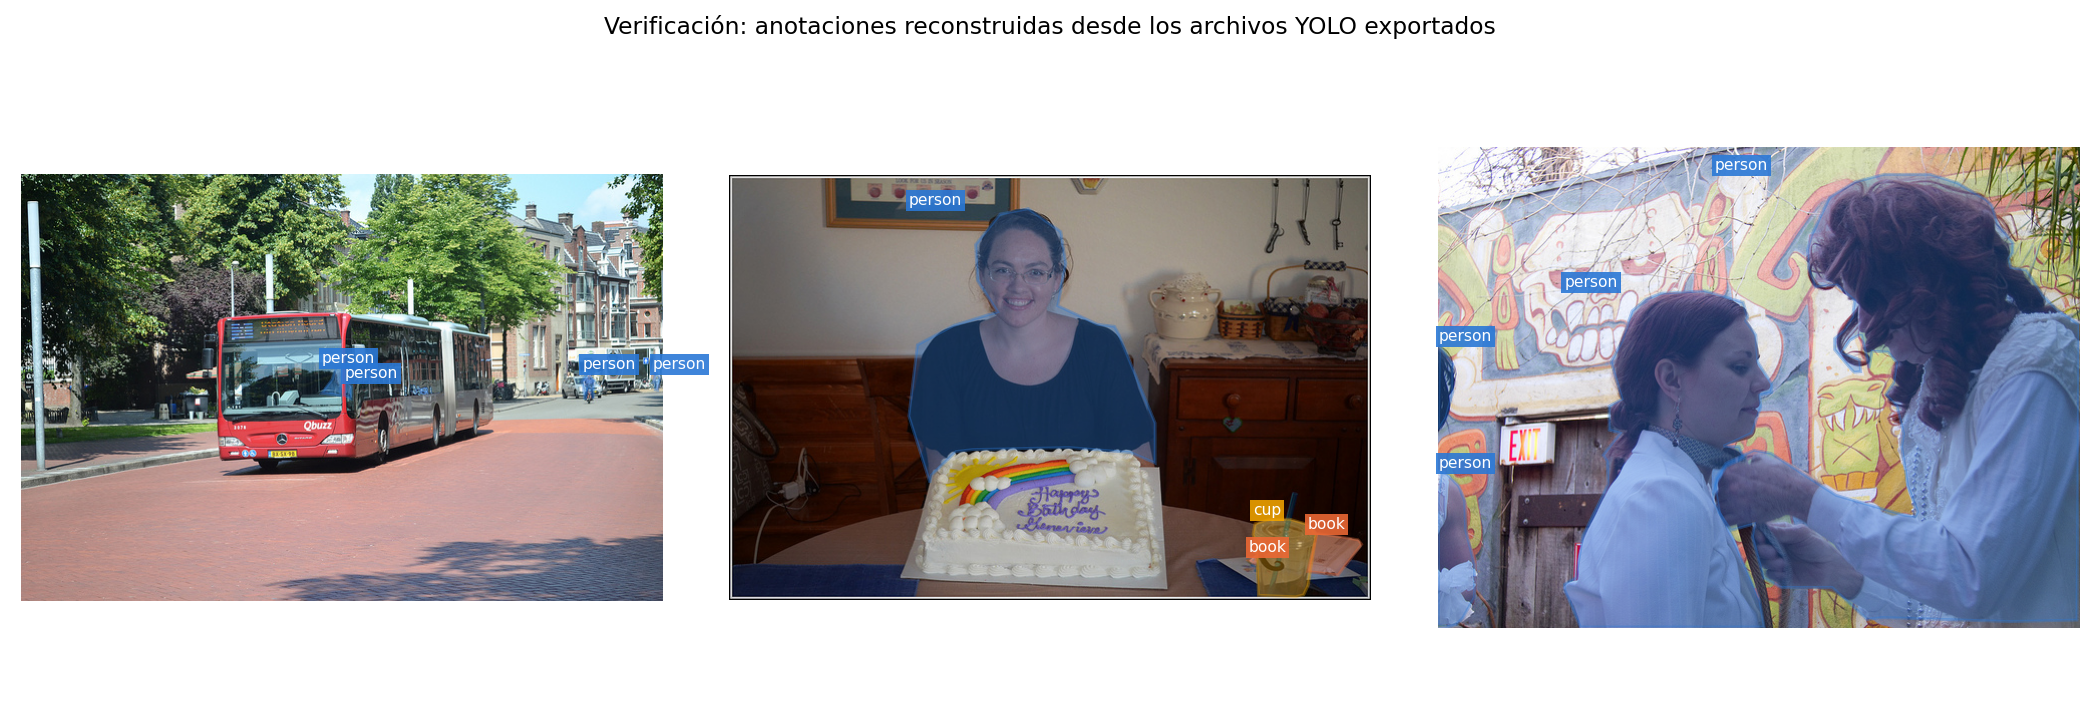
\includegraphics[width=\textwidth]{verificacion_etiquetas.png}
      \\[0.4em]
      {\scriptsize \textbf{Control de calidad:} las anotaciones se reconstruyen desde los
      archivos YOLO exportados y se superponen sobre las imágenes. Valida la cadena
      completa: formato, normalización de coordenadas y asignación de índices de clase.}
    \end{column}
  \end{columns}
\end{frame}

% ============================================================================
\section{Modelo y entrenamiento}

\begin{frame}{Arquitectura: YOLOv8n-seg}
  Modelo de segmentación de instancias de \textbf{una sola etapa} y \textbf{libre de anclas}.

  \vspace{0.5em}
  \begin{columns}[T]
    \begin{column}{0.55\textwidth}
      \begin{itemize}\footnotesize
        \item \textbf{Backbone} --- CSPDarknet con bloques C2f; extrae mapas de
              características a múltiples escalas.
        \item \textbf{Neck} --- PAN-FPN; fusiona semántica de alto nivel con detalle
              espacial de bajo nivel.
        \item \textbf{Cabeza desacoplada} --- predice caja, clase y un vector de
              \emph{coeficientes de máscara}; una rama paralela genera \emph{prototipos}
              de máscara (esquema derivado de YOLACT).
      \end{itemize}
      \vspace{0.4em}
      {\footnotesize La máscara de cada instancia es una \textbf{combinación lineal de los
      prototipos} $\Rightarrow$ costo de segmentación casi constante por imagen.}
    \end{column}
    \begin{column}{0.42\textwidth}
      \begin{block}{¿Por qué la variante \emph{nano}?}
        \footnotesize
        3,26~M de parámetros, 11,4~GFLOPs. Es la de menor capacidad de la familia.
        \vspace{0.4em}

        El requisito de tiempo real debe satisfacerse sobre la \textbf{CPU de una
        computadora personal}: es la variante con mejor relación
        desempeño--latencia para ese escenario.
      \end{block}
    \end{column}
  \end{columns}
\end{frame}

\begin{frame}{Transferencia de aprendizaje: qué se hereda y qué no}
  Se parte de los pesos preentrenados en COCO completo. Pero el vocabulario cambia de 80 a
  8 clases, y eso tiene una consecuencia que conviene explicitar:

  \vspace{0.5em}
  {\footnotesize\ttfamily\color{gris}
  Overriding model.yaml nc=80 with nc=8\\
  \color{rojo}Transferred 381/417 items from pretrained weights}

  \vspace{0.8em}
  \begin{columns}[T]
    \begin{column}{0.48\textwidth}
      \begin{exampleblock}{Se hereda}
        \footnotesize
        Backbone y neck completos: las representaciones visuales aprendidas sobre las
        118.000 imágenes de COCO.
      \end{exampleblock}
    \end{column}
    \begin{column}{0.48\textwidth}
      \begin{alertblock}{Se reinicializa}
        \footnotesize
        36 tensores ($\sim$372.000 parámetros): \textbf{toda la rama de clasificación de
        la cabeza} (\texttt{model.22.cv3}), cuyas dimensiones dependen de \texttt{nc}.
      \end{alertblock}
    \end{column}
  \end{columns}

  \vspace{0.8em}
  \begin{block}{Consecuencia de diseño}
    \footnotesize
    El clasificador arranca desde cero. Como el dominio de origen y el de destino
    \textbf{coinciden} (las 8 clases pertenecen a COCO), la estrategia es
    \textbf{congelar el backbone} y concentrar el presupuesto de optimización en la
    cabeza. Volveremos sobre esto en los resultados.
  \end{block}
\end{frame}

\begin{frame}{Preprocesamiento y aumento de datos}
  {\footnotesize
  \textbf{Preprocesamiento} (entrenamiento e inferencia): redimensionado a
  $640\times640$ por \emph{letterbox} (preserva la relación de aspecto, rellena con bordes
  neutros); intensidades normalizadas a $[0,1]$. \quad
  \textbf{Aumento} (solo entrenamiento): transforma de manera consistente las imágenes
  \emph{y} sus polígonos.}

  \vspace{0.4em}
  \begin{columns}[T]
    \begin{column}{0.60\textwidth}
      {\scriptsize
      \begin{tabular}{@{}llp{3.1cm}@{}}
        \toprule
        \textbf{Transformación} & \textbf{Valor} & \textbf{Justificación} \\
        \midrule
        \emph{Mosaic} & 1,0 & Contextos y escalas atípicos \\
        Volteo horizontal & $p{=}0{,}5$ & Sin quiralidad relevante \\
        Traslación & $\pm$10\,\% & Encuadres imperfectos \\
        Escala & $\pm$50\,\% & Distancia objeto--cámara \\
        HSV & $0{,}015 / 0{,}7 / 0{,}4$ & Iluminación y color \\
        \bottomrule
      \end{tabular}}

      \vspace{0.6em}
      {\scriptsize \emph{Mosaic} se desactiva en las últimas 10 épocas
      (\texttt{close\_mosaic}). \textbf{Se omiten} volteo vertical, rotaciones y
      \emph{mixup}: generarían poses inverosímiles para el dominio.}
    \end{column}
    \begin{column}{0.38\textwidth}
      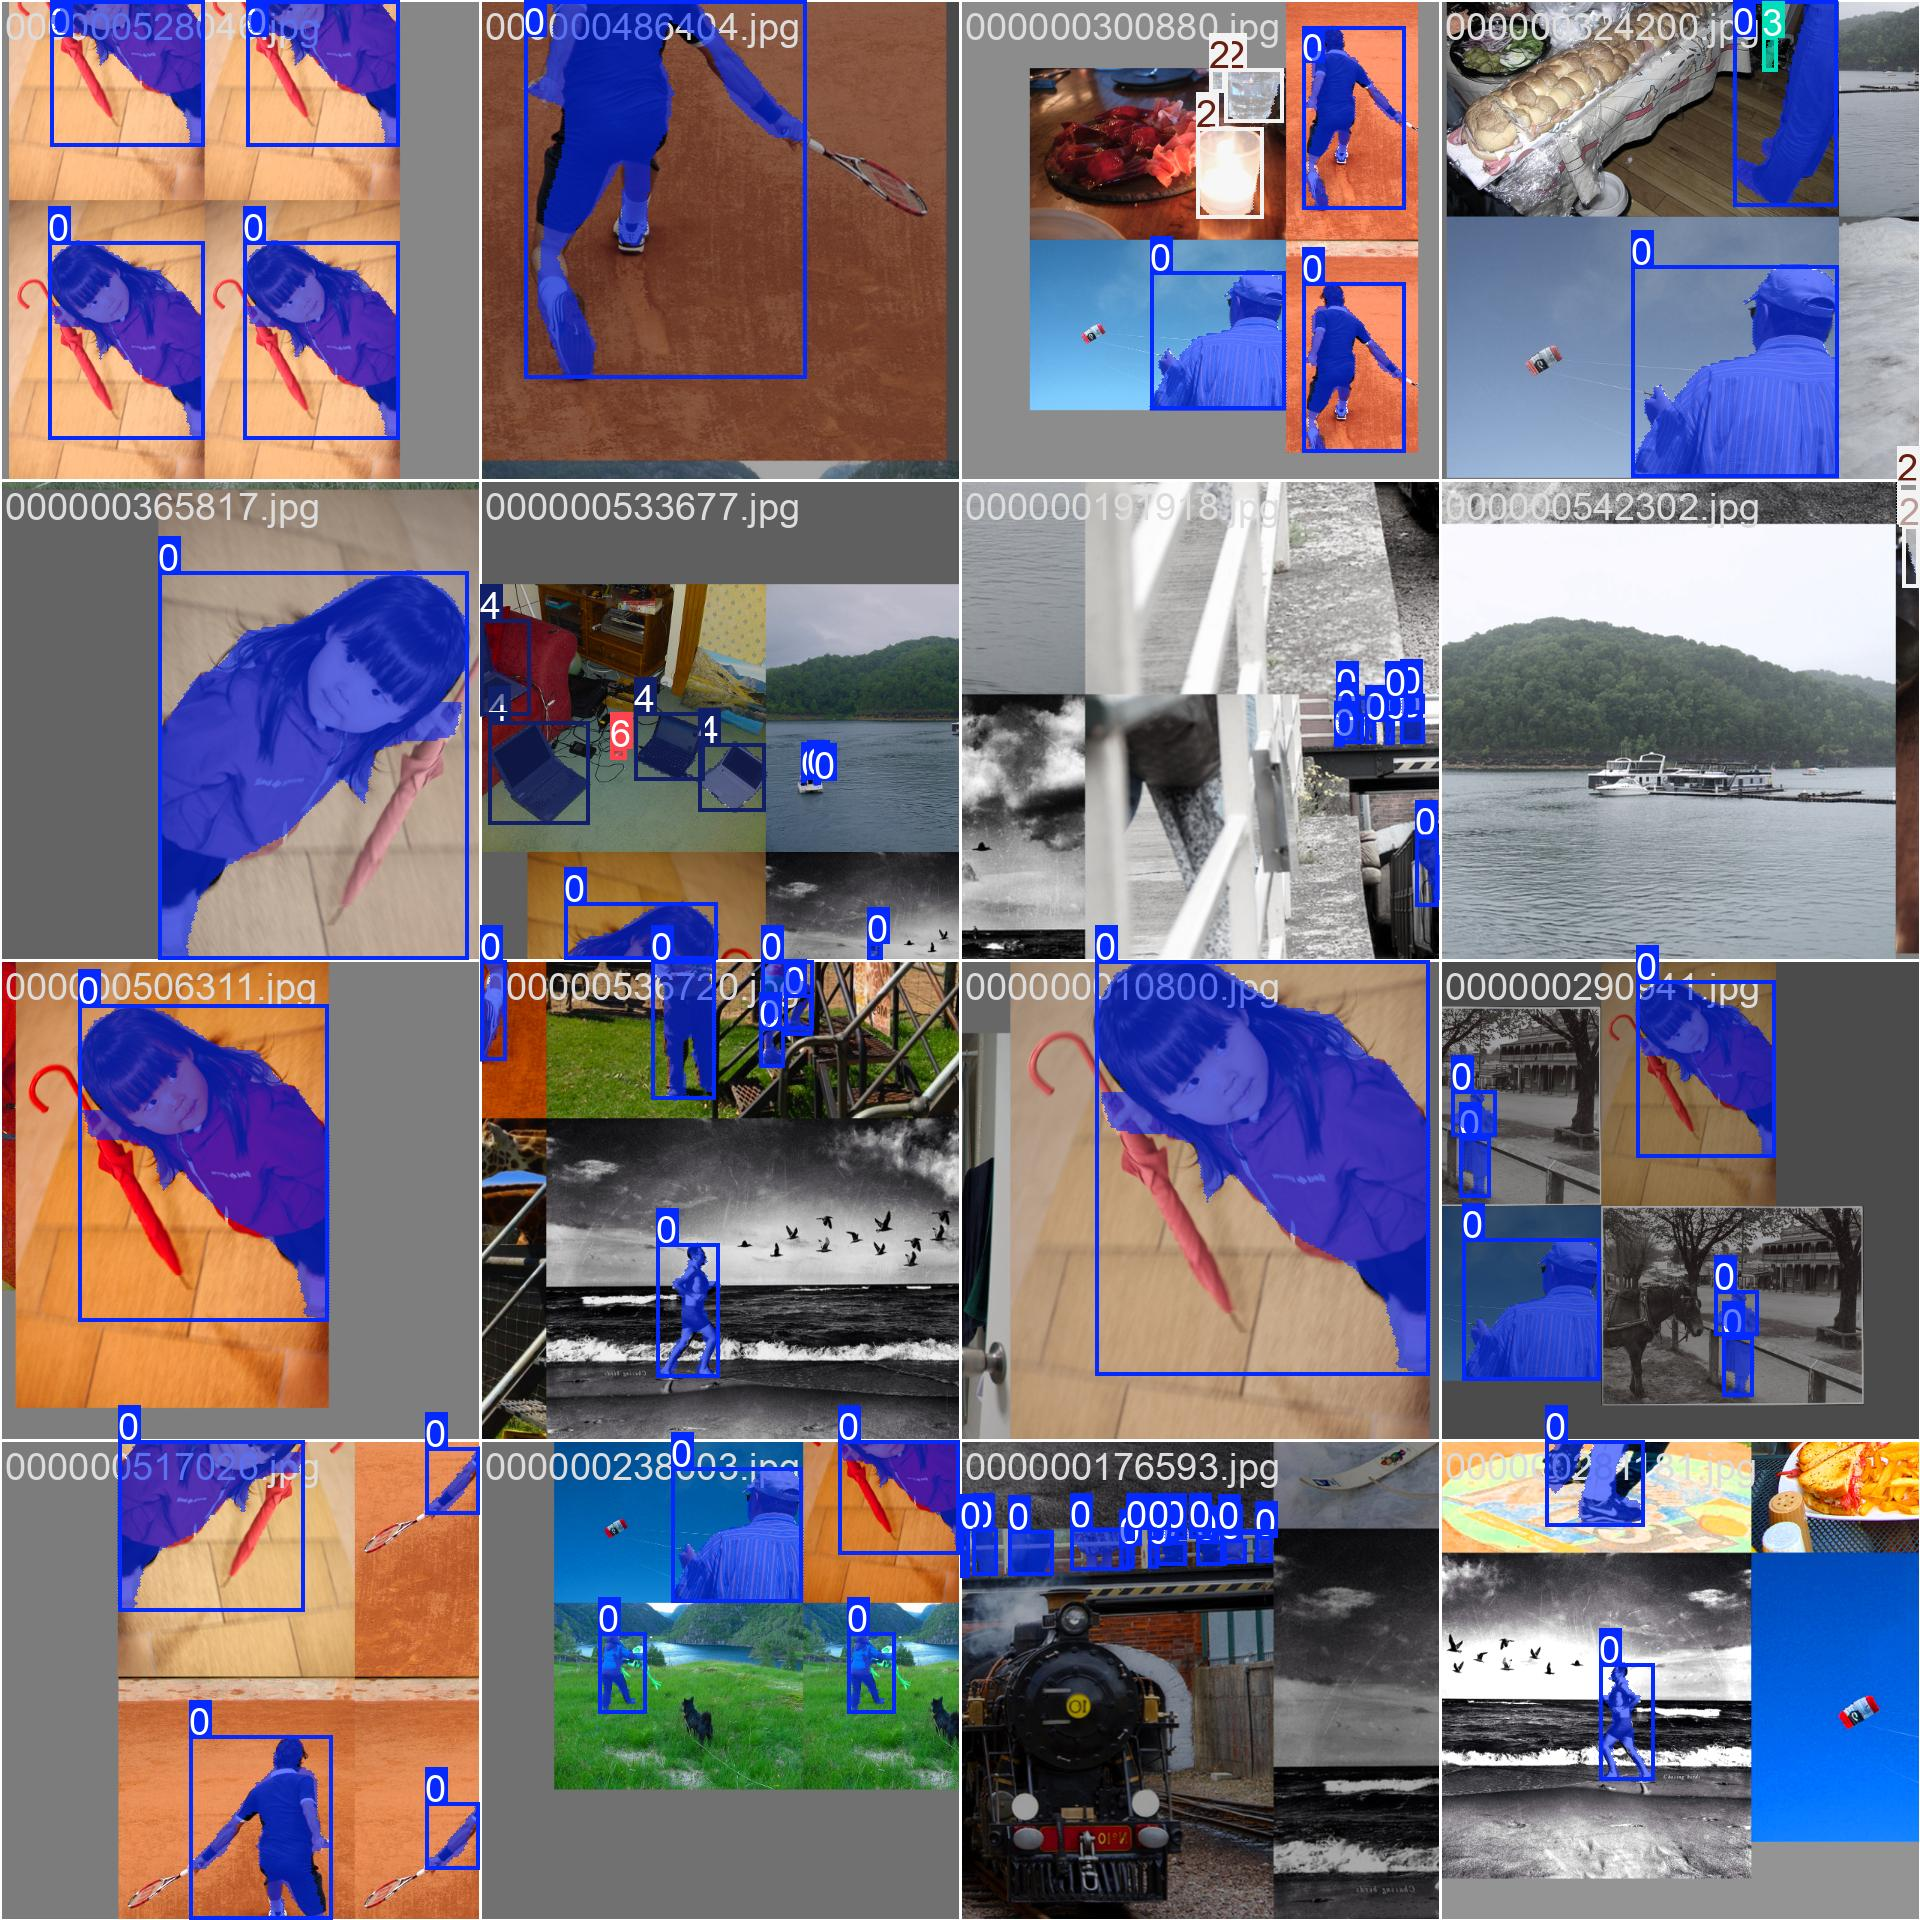
\includegraphics[width=0.86\textwidth]{mosaico_entrenamiento.jpg}
    \end{column}
  \end{columns}
\end{frame}

\begin{frame}{Configuración del entrenamiento}
  \centering
  \small
  \begin{tabular}{@{}ll@{}}
    \toprule
    \textbf{Parámetro} & \textbf{Valor} \\
    \midrule
    Modelo base & \texttt{yolov8n-seg.pt} (preentrenado en COCO) \\
    Capas congeladas & \texttt{freeze=10} (backbone); se entrenan neck y cabeza \\
    Épocas & 150 (early stopping, paciencia 50) \\
    Resolución de entrada & $640\times640$ (letterbox) \\
    Tamaño de lote & 32 \\
    Procesos de precarga & 4 \\
    Optimizador & AdamW (selección automática), $lr_0 = 8{,}33\times10^{-4}$, momento 0,9 \\
    Decaimiento de pesos & $5\times10^{-4}$ \\
    Precisión mixta (AMP) & Sí \\
    Semilla & 42 (modo determinista) \\
    Hardware & GPU NVIDIA RTX 5090 (32~GB) \\
    Duración & 132 minutos (se detuvo en la época 140) \\
    \bottomrule
  \end{tabular}

  \vspace{0.8em}
  {\footnotesize El lote y los procesos de precarga se fijaron explícitamente para acotar
  el consumo de memoria en un servidor compartido. El punto de control se selecciona por
  la \textbf{métrica de aptitud sobre validación}.}
\end{frame}

% ============================================================================
\section{Evaluación y resultados}

\begin{frame}{Protocolo de evaluación}
  \begin{columns}[T]
    \begin{column}{0.46\textwidth}
      \textbf{IoU} --- solapamiento entre la predicción $P$ y la anotación $G$:
      \begin{equation*}
        IoU(P,G) = \frac{|P \cap G|}{|P \cup G|}
      \end{equation*}
      Se aplica \textbf{tanto a cajas como a máscaras}. Una predicción es verdadero
      positivo si su IoU con una anotación de la misma clase supera un umbral.
      \vspace{0.6em}

      \textbf{AP} --- área bajo la curva precisión--recall de una clase.\\
      \textbf{mAP} --- promedio de las AP sobre las clases.
    \end{column}
    \begin{column}{0.5\textwidth}
      \begin{block}{Las dos variantes estándar}
        \footnotesize
        \textbf{mAP@50} --- umbral de IoU de 0,5. Criterio laxo: mide si el objeto fue
        encontrado.
        \vspace{0.4em}

        \textbf{mAP@50-95} --- promedio sobre umbrales de 0,5 a 0,95 en pasos de 0,05.
        Criterio estricto: premia la \textbf{precisión de la localización}. Es la métrica
        principal de este trabajo.
      \end{block}
      \vspace{0.4em}
      {\footnotesize Todo se calcula por separado para \textbf{cajas} (detección) y
      \textbf{máscaras} (segmentación), sobre la partición de prueba
      (1.250 imágenes, 7.117 instancias), reservada de principio a fin.}
    \end{column}
  \end{columns}
\end{frame}

\begin{frame}{Curvas de aprendizaje}
  \centering
  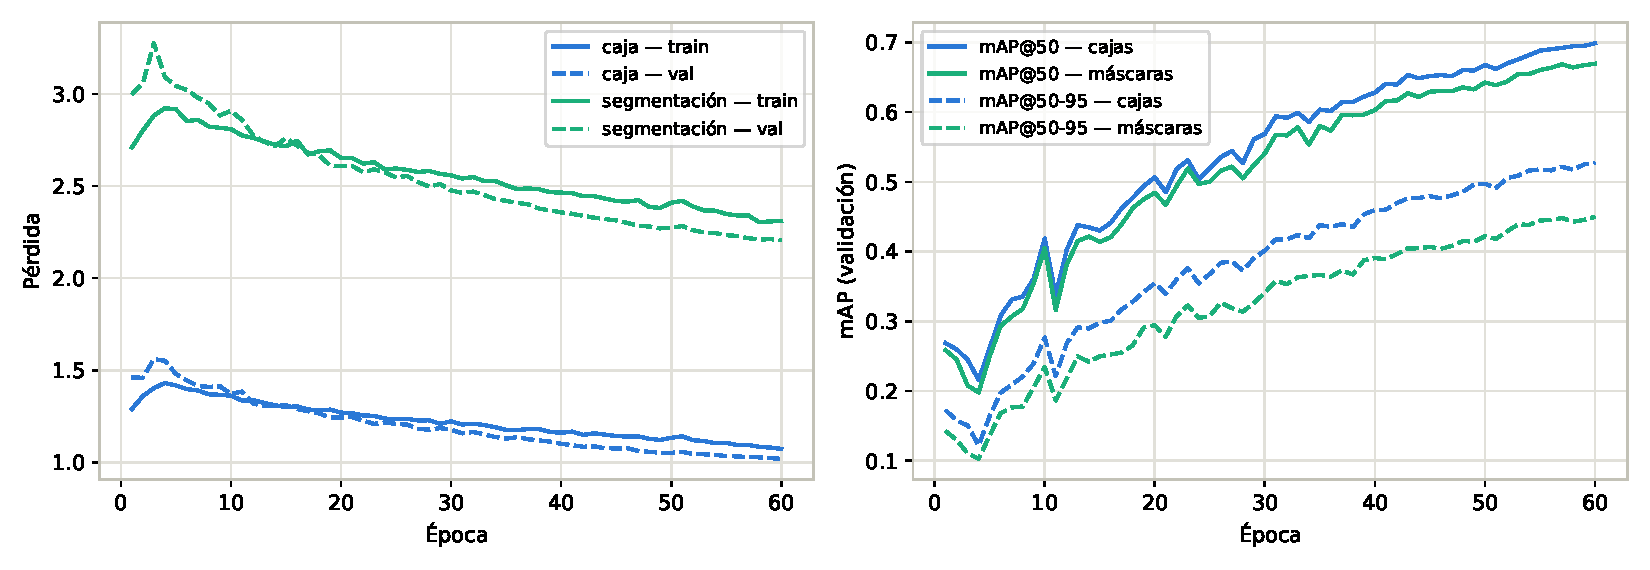
\includegraphics[width=0.92\textwidth]{curvas_entrenamiento.pdf}

  \vspace{0.4em}
  \begin{itemize}\footnotesize
    \item Las pérdidas de caja y segmentación decrecen de forma sostenida, sin
          divergencia: no hay sobreajuste.
    \item El mAP de validación crece rápido y se estabiliza en una meseta (mAP@50-95 de
          máscaras hasta 0,283), coherente con un modelo de \emph{backbone} congelado.
    \item La pérdida de validación se ubica \textbf{por encima} de la de entrenamiento,
          como corresponde a la brecha de generalización sobre una partición reservada.
  \end{itemize}
\end{frame}

\begin{frame}{Métricas sobre la partición de prueba}
  \centering
  \small
  \begin{tabular}{@{}lcc@{}}
    \toprule
    \textbf{Métrica} & \textbf{Cajas (detección)} & \textbf{Máscaras (segmentación)} \\
    \midrule
    Precisión media & 0,577 & 0,559 \\
    Recall medio    & 0,397 & 0,383 \\
    mAP@50          & 0,440 & 0,420 \\
    mAP@50-95       & \textbf{0,292} & \textbf{0,246} \\
    \bottomrule
  \end{tabular}

  \vspace{0.8em}
  \begin{columns}
    \begin{column}{0.48\textwidth}
      \begin{block}{El recall es el cuello de botella}
        \footnotesize
        La precisión (0,577) supera con holgura al recall (0,397): el modelo acierta
        cuando detecta, pero \textbf{omite} muchas instancias.
      \end{block}
    \end{column}
    \begin{column}{0.48\textwidth}
      \begin{block}{Máscaras por debajo de cajas}
        \footnotesize
        El IoU a nivel de píxel es más estricto que el de rectángulos, sobre todo en
        contornos complejos como los de \texttt{person}.
      \end{block}
    \end{column}
  \end{columns}

  \vspace{0.4em}
  {\scriptsize \footnotesize Estos valores se interpretan frente al baseline en la
  comparación imparcial (dos láminas más adelante).}
\end{frame}

\begin{frame}{Desempeño por clase}
  \centering
  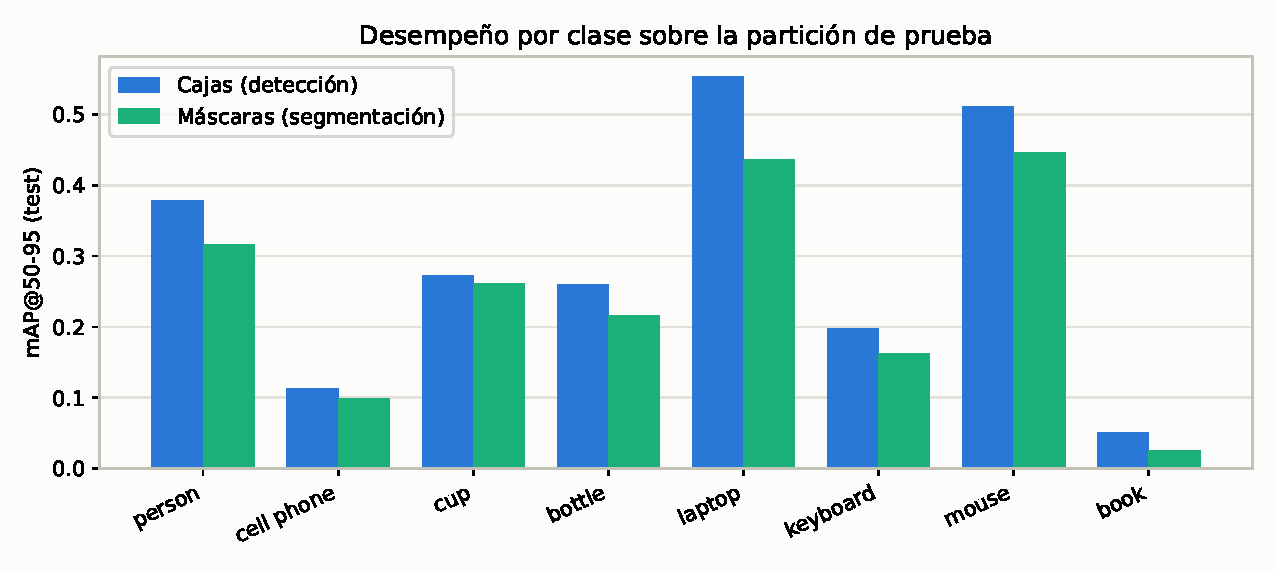
\includegraphics[width=0.68\textwidth]{map_por_clase.pdf}

  \vspace{0.3em}
  \begin{columns}
    \begin{column}{0.48\textwidth}
      \begin{exampleblock}{Mejores clases: \texttt{laptop}, \texttt{mouse}}
        \footnotesize
        mAP@50-95 de cajas de 0,554 y 0,512. Objetos rígidos, de contorno regular, poco
        ocluidos.
      \end{exampleblock}
    \end{column}
    \begin{column}{0.48\textwidth}
      \begin{alertblock}{Peor clase: \texttt{book}}
        \footnotesize
        En COCO aparecen apilados o en estanterías: instancias pequeñas, con límites
        ambiguos y anotación inconsistente.
      \end{alertblock}
    \end{column}
  \end{columns}
\end{frame}

\begin{frame}{Matriz de confusión: ¿dónde falla el modelo?}
  \begin{columns}[T]
    \begin{column}{0.52\textwidth}
      \centering
      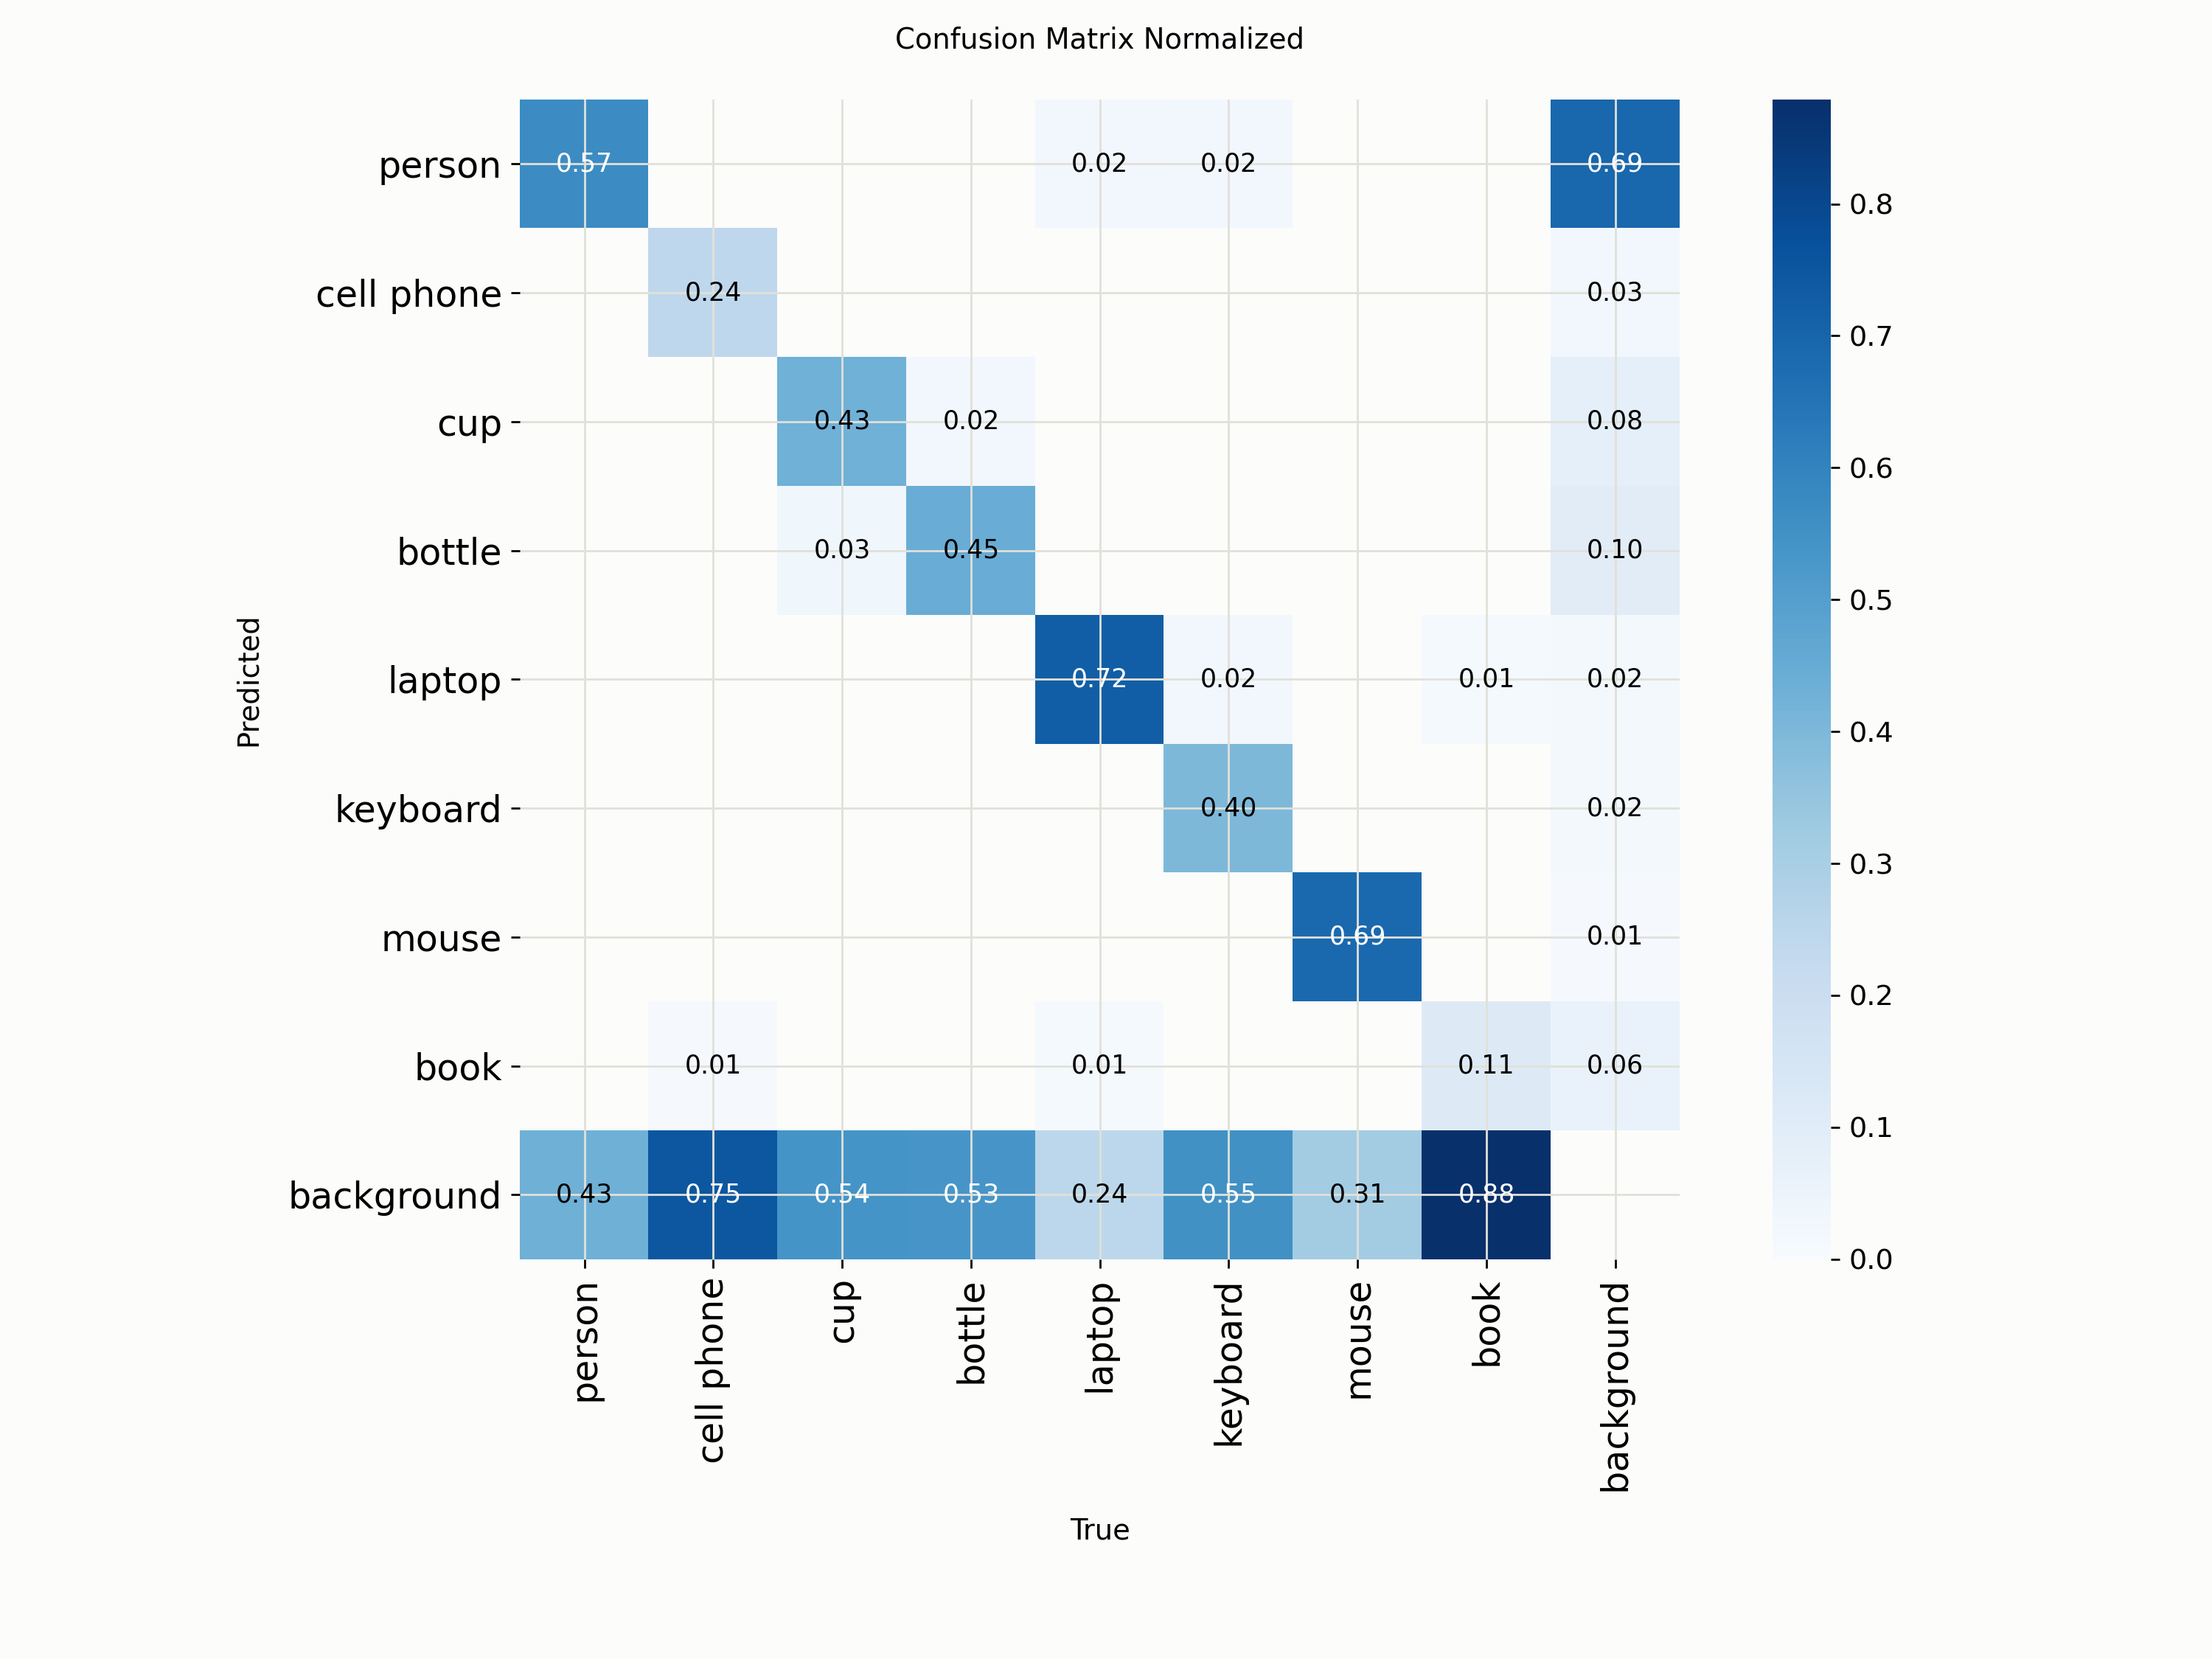
\includegraphics[width=\textwidth]{confusion_matrix.png}
    \end{column}
    \begin{column}{0.44\textwidth}
      \begin{block}{Hallazgo}
        \footnotesize
        El modelo \textbf{prácticamente no confunde clases entre sí} (máximo 0,03). El modo
        de error dominante es la \textbf{omisión}: objetos reales clasificados como fondo.
      \end{block}
      \vspace{0.5em}
      \begin{itemize}\footnotesize
        \item El vocabulario reducido hace que la \emph{clasificación} sea sencilla.
        \item El desafío restante es la \emph{detección} de instancias pequeñas u
              ocluidas.
        \item[$\Rightarrow$] El margen de mejora está en el \textbf{recall}, no en la
              discriminación.
      \end{itemize}
      \vspace{0.4em}
      {\scriptsize Omisión por clase: \texttt{book} 88\,\%, \texttt{cell phone} 75\,\%,
      \texttt{keyboard} 55\,\%, \texttt{cup} 54\,\%, \texttt{bottle} 53\,\%.}
    \end{column}
  \end{columns}
\end{frame}

\begin{frame}{El sesgo oculto en la comparación con el baseline}
  Comparar el modelo ajustado (0,246 de máscaras) contra el preentrenado sobre nuestra
  partición de prueba sugiere que el preentrenado gana (0,342). \textbf{Pero esa
  comparación es tramposa.}

  \vspace{0.6em}
  \begin{alertblock}{El baseline ya vio nuestro test}
    \footnotesize
    El modelo preentrenado (\texttt{yolov8n-seg.pt}) se entrenó sobre COCO~\textbf{train2017},
    el mismo conjunto del que muestreamos nuestras 5.000 imágenes. Es decir: el baseline
    fue entrenado sobre las mismas imágenes que aquí usamos como prueba, mientras que
    nuestro modelo se evalúa sobre datos genuinamente reservados.
  \end{alertblock}

  \vspace{0.4em}
  \begin{exampleblock}{La corrección: evaluar sobre COCO val2017}
    \footnotesize
    Se construyó una partición de prueba independiente desde \textbf{COCO val2017} ---el
    conjunto de validación oficial, que el preentrenado nunca usó para ajustar sus pesos y
    es disjunto de train2017. Sobre esas 1.250 imágenes, \emph{ninguno} de los dos modelos
    vio los datos: la comparación es limpia.
  \end{exampleblock}
\end{frame}

\begin{frame}{Comparación imparcial sobre COCO val2017}
  \begin{columns}[T]
    \begin{column}{0.56\textwidth}
      \centering
      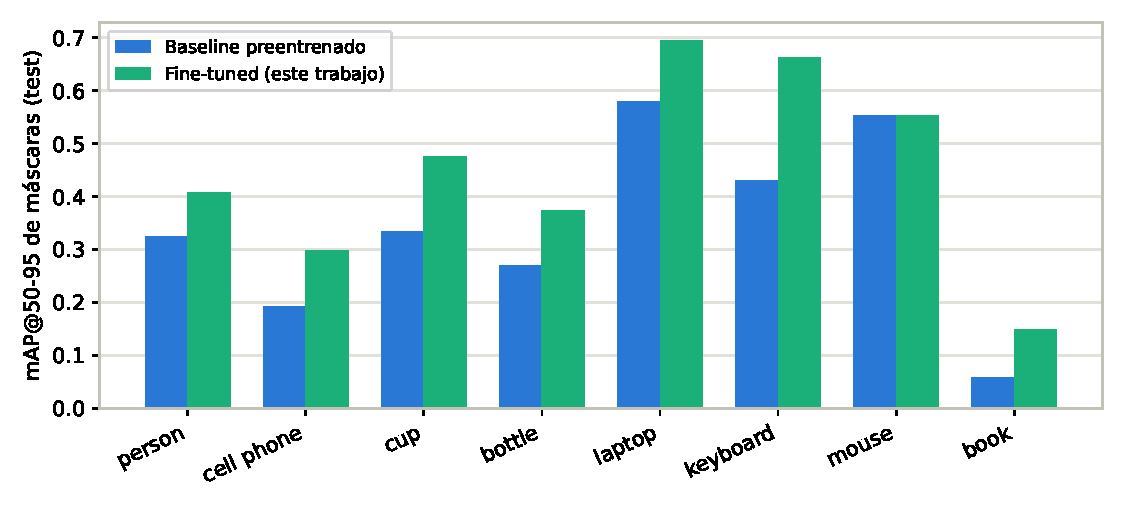
\includegraphics[width=\textwidth]{baseline_vs_finetuned.pdf}
    \end{column}
    \begin{column}{0.42\textwidth}
      \footnotesize
      \begin{tabular}{@{}lcc@{}}
        \toprule
        mAP@50-95 & Base & Ajust. \\
        \midrule
        Máscaras & 0,277 & 0,236 \\
        Cajas & 0,329 & 0,275 \\
        \bottomrule
      \end{tabular}
      \vspace{0.6em}

      Al pasar a datos no vistos, el baseline \textbf{cae} de 0,342 a 0,277; nuestro modelo
      apenas varía (0,246 $\to$ 0,236).
      \vspace{0.4em}

      \textbf{Dos tercios de la brecha aparente} eran la ventaja de fuga del baseline. Bajo
      la comparación justa hay \textbf{paridad} en \texttt{person} ($-$0,008) y
      \texttt{mouse} ($-$0,007).
    \end{column}
  \end{columns}

  \vspace{0.3em}
  \begin{block}{Por qué el preentrenado es un baseline tan fuerte}
    \footnotesize
    Las 8 clases son un \textbf{subconjunto} de su vocabulario: las aprendió sobre 118.000
    imágenes. Ajustar sobre 3.000 del mismo dominio no agrega información nueva; lo
    esperable es igualarlo, no superarlo en mAP.
  \end{block}
\end{frame}

\begin{frame}{Ablación: ajuste fino completo frente a backbone congelado}
  \begin{block}{El experimento que motivó la configuración final}
    \footnotesize
    Un ajuste fino \textbf{completo} (sin congelar capas, 60 épocas) sobre 3.000 imágenes
    quedó \emph{por debajo} del modelo preentrenado sin tocar. La causa es la
    reinicialización de la cabeza de clasificación: 372.000 parámetros que deben
    reaprenderse con dos órdenes de magnitud menos de datos que en el preentrenamiento.
  \end{block}

  \vspace{0.5em}
  \centering
  \small
  \begin{tabular}{@{}lcc@{}}
    \toprule
    \textbf{Configuración} & \textbf{mAP@50-95 cajas} & \textbf{mAP@50-95 máscaras} \\
    \midrule
    Ajuste fino completo, 60 épocas & 0,250 & 0,216 \\
    \textbf{Backbone congelado, 150 épocas} & \textbf{0,292} & \textbf{0,246} \\
    \bottomrule
  \end{tabular}

  \vspace{0.3em}
  {\scriptsize (métricas sobre la partición de prueba de train2017)}

  \vspace{0.6em}
  \begin{exampleblock}{Lección}
    \footnotesize
    Cuando el vocabulario de destino es un \textbf{subconjunto} del de preentrenamiento, un
    ajuste fino ingenuo con la cabeza reinicializada puede \emph{degradar} el modelo.
    Congelar el backbone recupera parte de la brecha y vuelve \textbf{segura} la
    transferencia.
  \end{exampleblock}
\end{frame}

\begin{frame}{Análisis cualitativo: el verdadero aporte del ajuste}
  \begin{columns}[T]
    \begin{column}{0.5\textwidth}
      \centering {\scriptsize Baseline (80 clases)}\\
      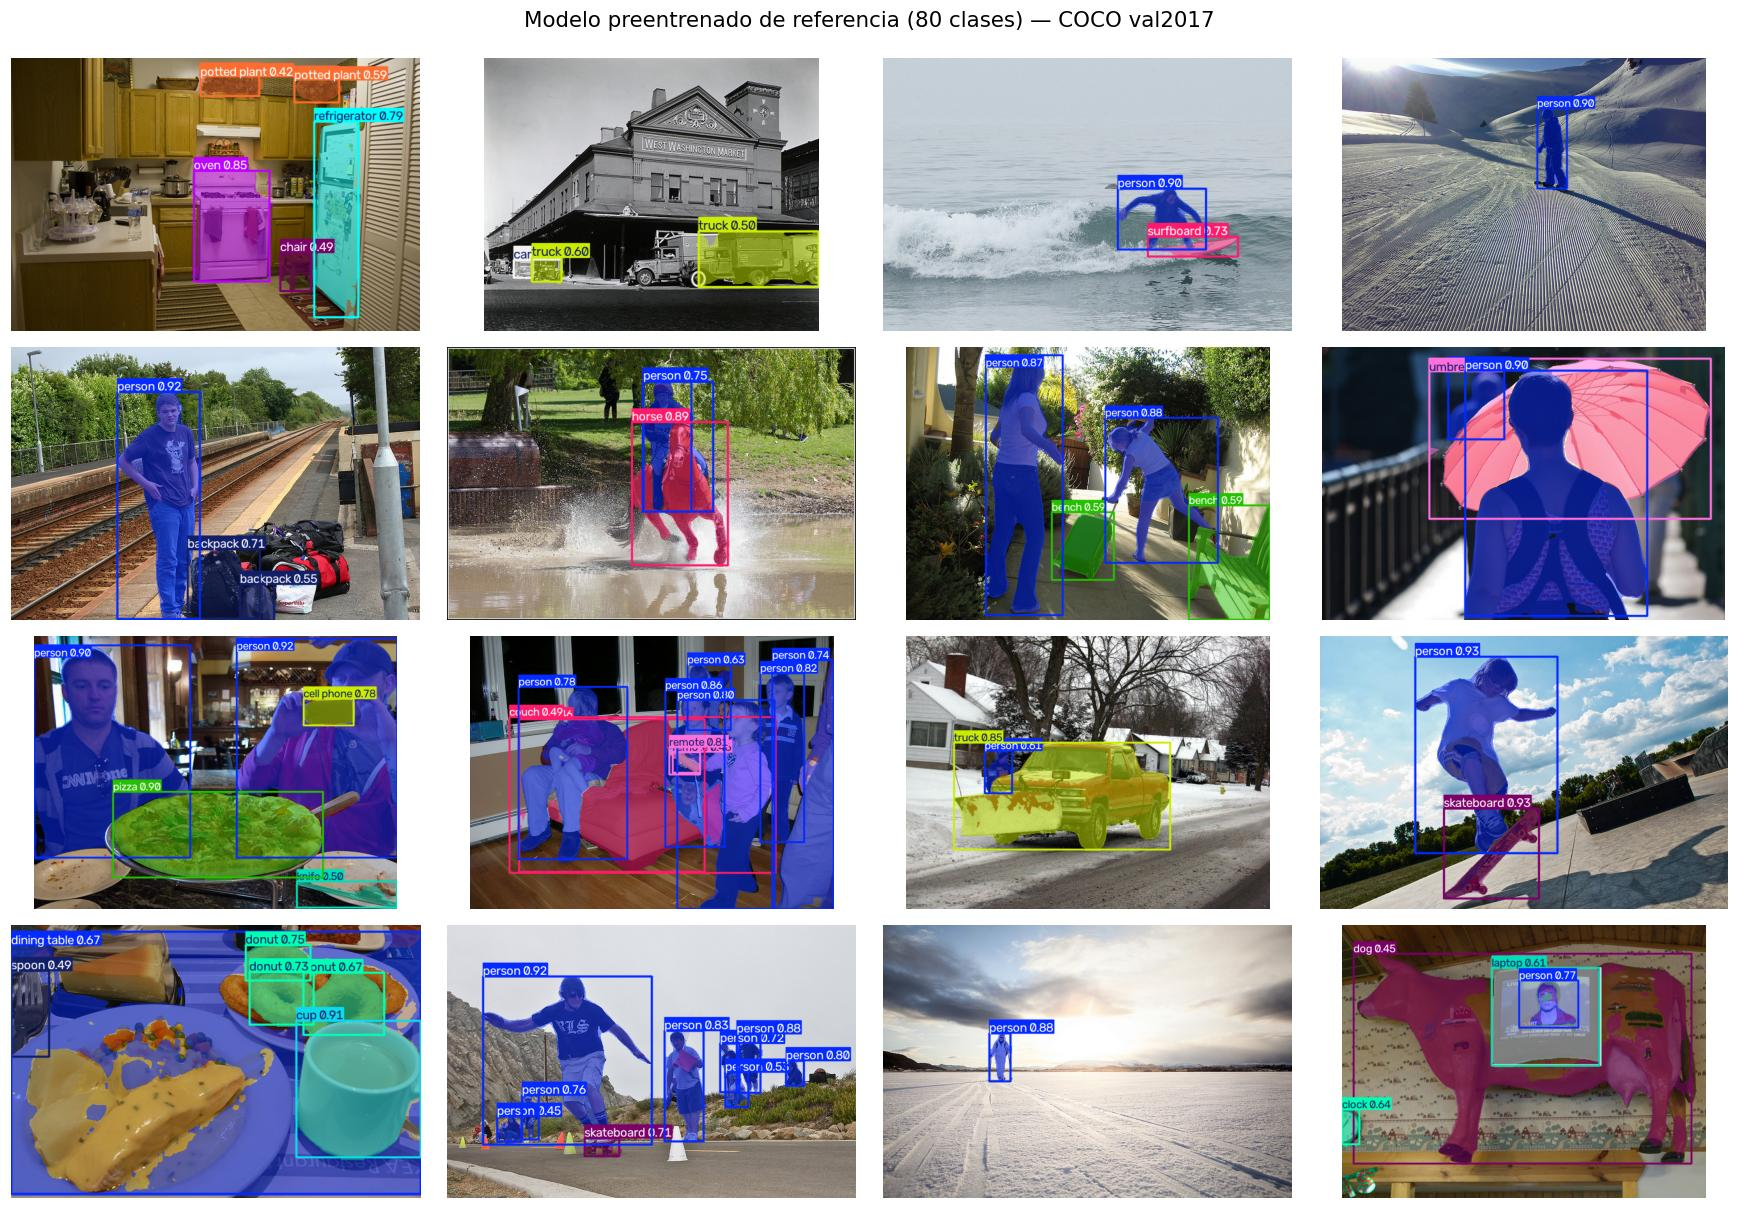
\includegraphics[width=\textwidth]{cualitativo_baseline.jpg}
    \end{column}
    \begin{column}{0.5\textwidth}
      \centering {\scriptsize Ajustado (8 clases)}\\
      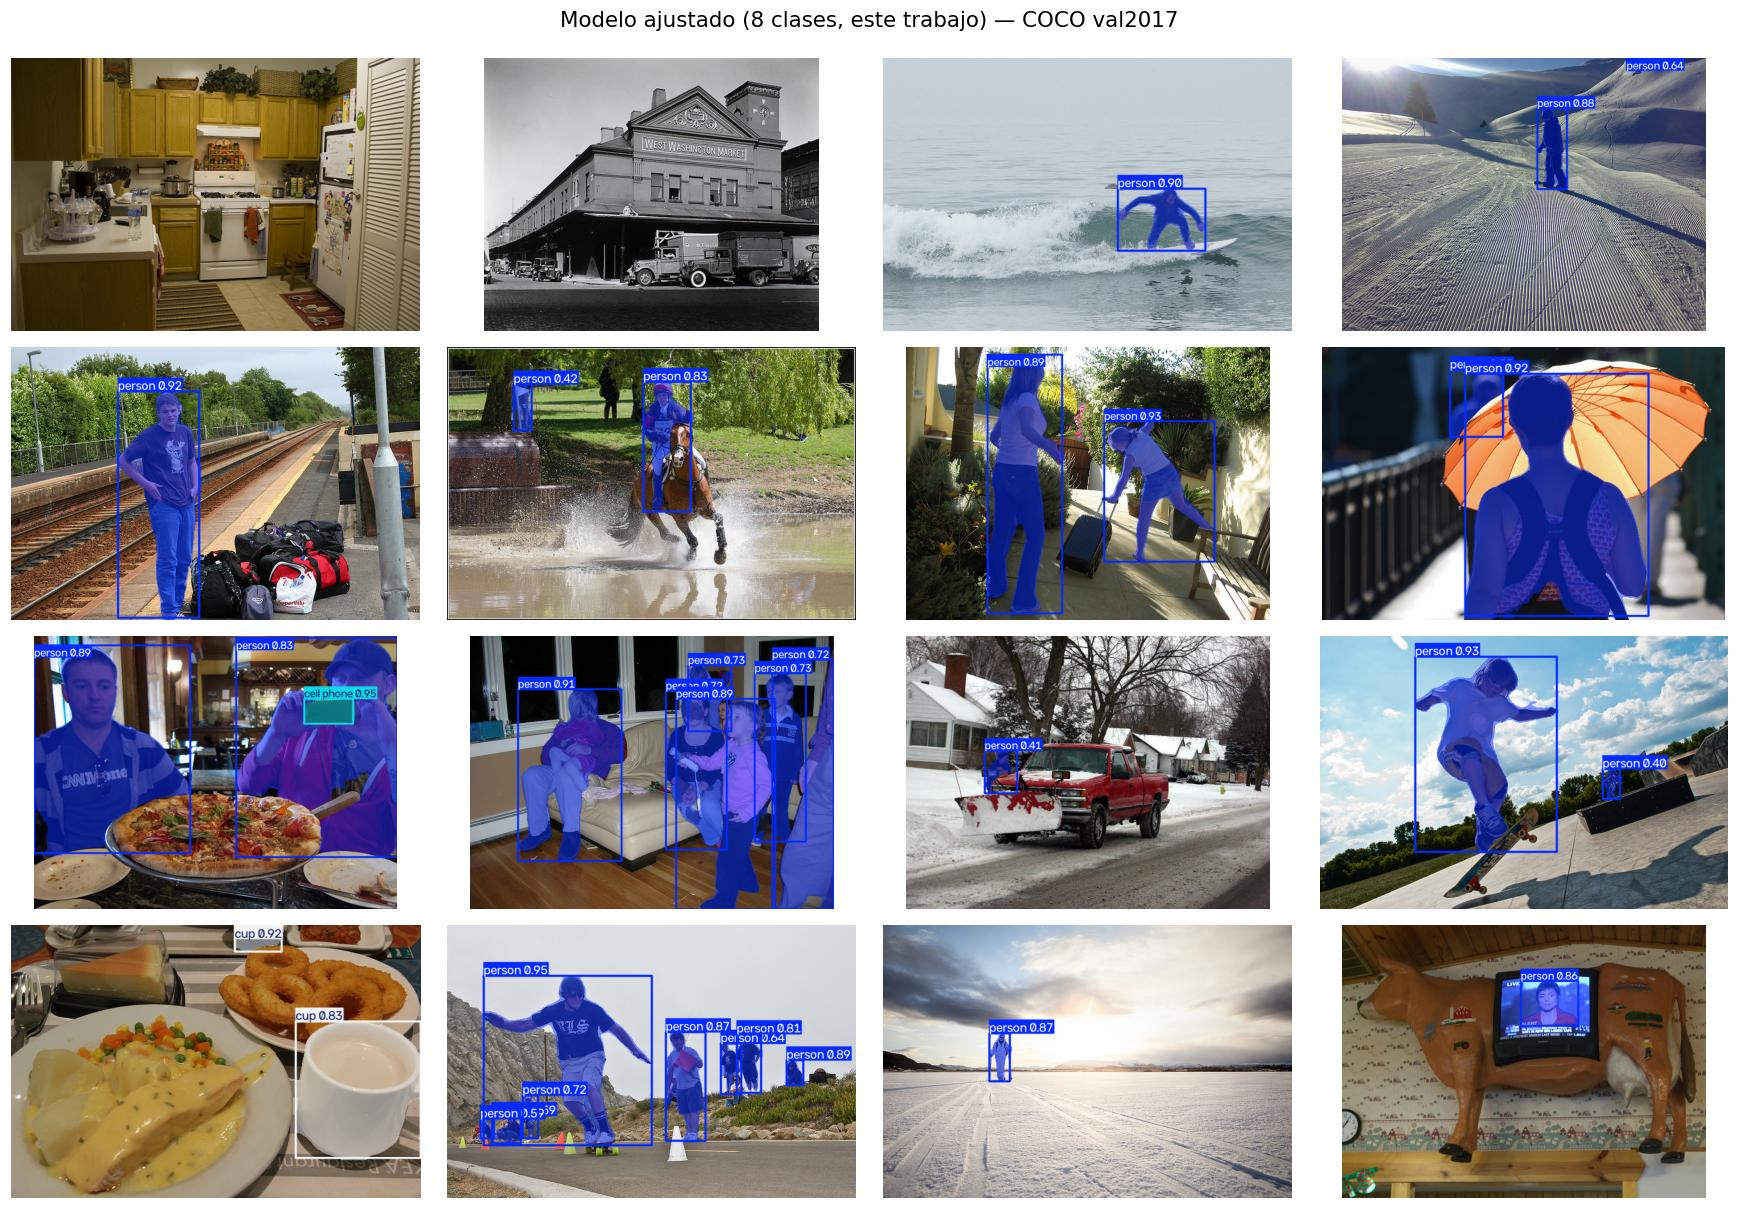
\includegraphics[width=\textwidth]{cualitativo_finetuned.jpg}
    \end{column}
  \end{columns}

  \vspace{0.3em}
  \begin{itemize}\footnotesize
    \item El baseline dispersa detecciones fuera de alcance
          (\texttt{refrigerator}, \texttt{surfboard}, \texttt{horse}, \texttt{umbrella},
          \texttt{pizza}, \texttt{cow}\ldots).
    \item El ajustado se concentra \textbf{exclusivamente} en las 8 clases: suprime por
          completo los falsos positivos de vocabulario. \emph{Esta} es su ventaja práctica,
          invisible al mAP por clase.
  \end{itemize}
\end{frame}

% ============================================================================
\section{Sistema en tiempo real}

\begin{frame}[fragile]{Implementación de la inferencia en tiempo real}
  \texttt{src/demo\_webcam.py}: captura por OpenCV, inferencia cuadro a cuadro y
  superposición de cajas, máscaras, etiquetas con confianza y FPS.

  \vspace{0.5em}
\begin{lstlisting}[style=py]
modelo = YOLO(args.model, task='segment')     # pesos .pt o modelo OpenVINO
captura = cv2.VideoCapture(fuente)            # webcam (índice) o archivo

while True:
    ok, fotograma = captura.read()
    resultados = modelo.predict(fotograma, conf=args.conf, imgsz=args.imgsz)
    anotado = resultados[0].plot()            # cajas + máscaras + etiquetas
    cv2.imshow(ventana, anotado)
\end{lstlisting}

  \vspace{0.4em}
  \begin{itemize}\footnotesize
    \item FPS suavizados con media móvil exponencial (lectura estable).
    \item Fuente de video, umbral de confianza y resolución de inferencia configurables
          por línea de comandos.
    \item La computadora de demostración \textbf{no tiene GPU con CUDA} $\Rightarrow$
          se exporta el modelo a \textbf{OpenVINO} (representación intermedia de Intel,
          especializada para CPU y gráficos integrados).
  \end{itemize}
\end{frame}

\begin{frame}{Desempeño medido}
  \centering
  \small
  \begin{tabular}{@{}llcc@{}}
    \toprule
    \textbf{Plataforma} & \textbf{Formato} & \textbf{Latencia} & \textbf{FPS} \\
    \midrule
    Servidor, GPU RTX 5090 & PyTorch (\texttt{.pt}) & 5,1 ms/imagen & $\sim$198 \\
    PC personal, CPU Core Ultra 5 & PyTorch (\texttt{.pt}) & $\sim$59 ms/cuadro & 17 \\
    PC personal, CPU Core Ultra 5 & OpenVINO & $\sim$29 ms/cuadro & \textbf{35} \\
    \bottomrule
  \end{tabular}

  \vspace{0.3em}
  \begin{columns}
    \begin{column}{0.36\textwidth}
      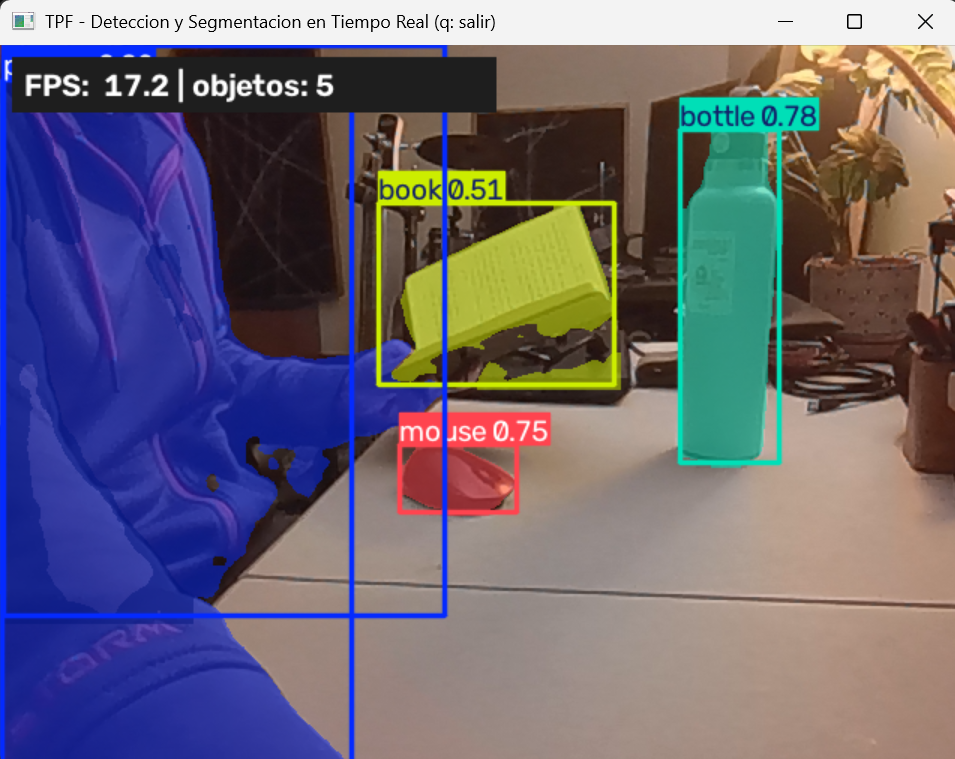
\includegraphics[width=\textwidth]{webcam_pt.png}\\
      \centering{\scriptsize PyTorch: 17,2 FPS}
    \end{column}
    \begin{column}{0.36\textwidth}
      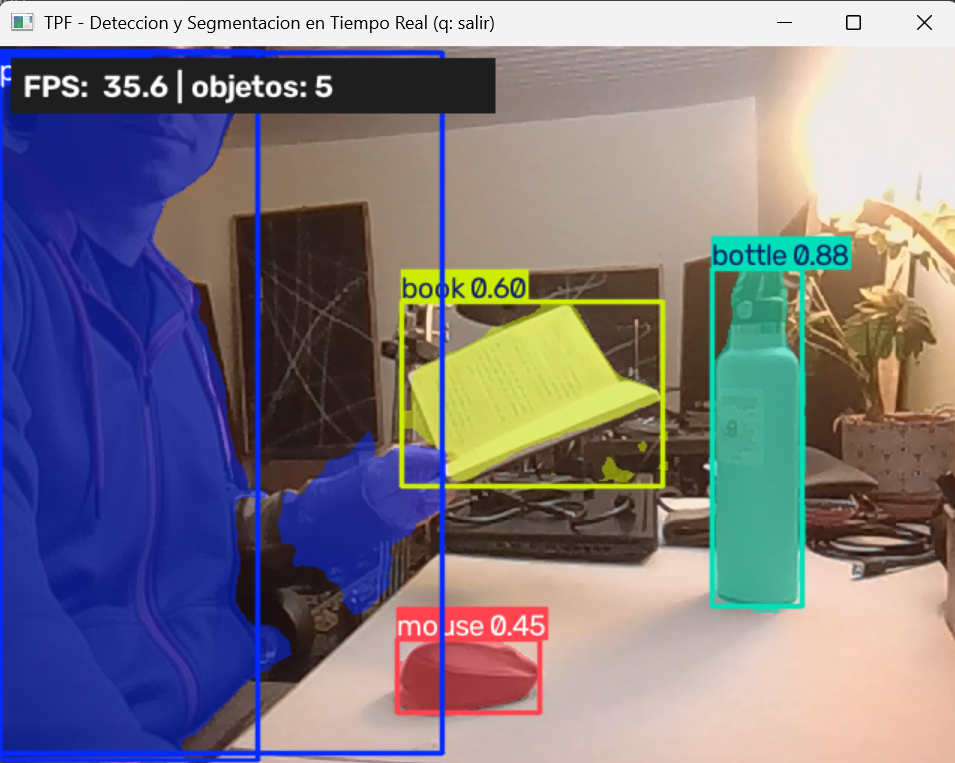
\includegraphics[width=\textwidth]{webcam_openvino.png}\\
      \centering{\scriptsize OpenVINO: 35,6 FPS}
    \end{column}
  \end{columns}

  \vspace{0.2em}
  \centering{\scriptsize OpenVINO \textbf{duplica} la tasa de cuadros y supera el umbral de
  tiempo real (24--30 FPS) sin aceleración dedicada.}
\end{frame}

\begin{frame}{Despliegue en la nube: Hugging Face Spaces}
  \begin{columns}[T]
    \begin{column}{0.46\textwidth}
      La aplicación se desplegó en un \textbf{servidor público} con interfaz Gradio: quien
      la evalúe solo abre un enlace, sin descargar ni instalar nada.
      \vspace{0.6em}

      \textbf{Dos modos de uso}
      \begin{itemize}\footnotesize
        \item \textbf{Imagen} --- sube una fotografía; devuelve cajas, máscaras y recuento
              de objetos por clase.
        \item \textbf{Webcam en vivo} --- inferencia cuadro a cuadro sobre la cámara del
              navegador, con umbral de confianza y resolución expuestos.
      \end{itemize}
      \vspace{0.6em}
      {\scriptsize Los pesos viajan dentro del repositorio del Space: el modelo se ejecuta
      íntegramente en la nube.}
    \end{column}
    \begin{column}{0.5\textwidth}
      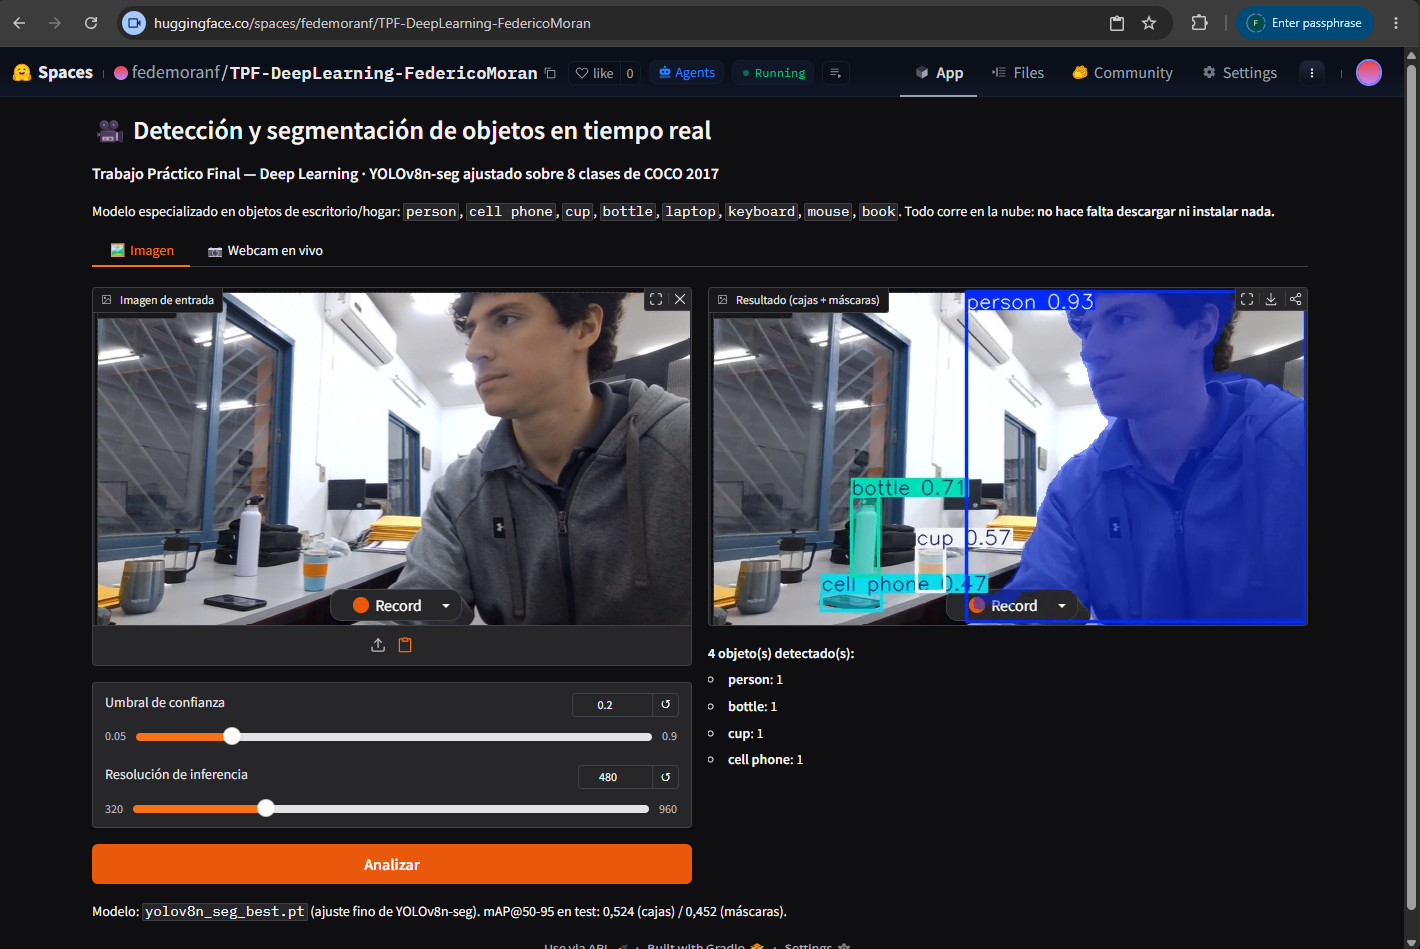
\includegraphics[width=\textwidth]{prueba_huggingface.png}
    \end{column}
  \end{columns}
\end{frame}

\begin{frame}[plain]
  \centering
  \vfill
  {\Huge\bfseries\color{azul} Demostración en vivo}
  \vfill
  {\large Detección y segmentación de instancias sobre cámara web}\\[0.5em]
  {\normalsize CPU Intel Core Ultra 5 226V --- sin GPU dedicada}
  \vfill
\end{frame}

% ============================================================================
\section{Conclusiones}

\begin{frame}{Limitaciones}
  \begin{itemize}
    \item \textbf{Desbalance de clases.} \texttt{person} concentra el 74,2\,\% de las
          instancias; \texttt{mouse} y \texttt{keyboard} tienen menos de 150 ejemplos de
          entrenamiento. No se corrigió de forma artificial; se tiene presente al
          interpretar las métricas por clase.
    \item \textbf{Calidad de la anotación de referencia.} La categoría \texttt{book} tiene
          límites ambiguos en COCO, lo que impone un techo a su desempeño medible.
    \item \textbf{Pérdida por simplificación de polígonos.} La conversión máscara
          $\rightarrow$ polígono (tolerancia 2~px) y el descarte de fragmentos degenerados
          eliminan $\sim$4\,\% de las líneas de anotación.
    \item \textbf{Escala del conjunto de datos.} 3.000 imágenes de entrenamiento son dos
          órdenes de magnitud menos que el preentrenamiento de COCO; esa es precisamente
          la razón por la que congelar el backbone resulta determinante.
  \end{itemize}
\end{frame}

\begin{frame}{Conclusiones}
  \begin{enumerate}
    \item \textbf{La evaluación rigurosa es tan determinante como el modelo.} Se
          corrigieron dos sesgos optimistas ---la fuga en el propio \emph{split} y el
          preentrenamiento del baseline sobre el mismo pozo de datos---; bajo una
          comparación imparcial en val2017 el modelo ajustado es competitivo con el
          preentrenado, y su aporte real es la especialización, no el mAP.
    \vspace{0.3em}
    \item \textbf{El desempeño por clase está gobernado por las características visuales y
          la calidad de anotación de cada categoría}, no por la confusión entre clases: la
          matriz de confusión muestra que el error dominante es la omisión de instancias
          pequeñas u ocluidas.
    \vspace{0.3em}
    \item \textbf{La segmentación de instancias en tiempo real es viable sobre una CPU de
          consumo.} La variante nano exportada a OpenVINO alcanzó 35~FPS sostenidos sin GPU
          dedicada, el doble que el formato PyTorch original.
    \vspace{0.3em}
    \item \textbf{El pipeline resultó reproducible de extremo a extremo}, con semillas
          fijas y controles de integridad que verifican, sobre los archivos exportados, que
          las particiones sean disjuntas.
  \end{enumerate}
\end{frame}

\begin{frame}{Trabajo futuro}
  \begin{itemize}
    \item \textbf{Ampliar el conjunto de datos}, en particular para las clases raras
          (\texttt{keyboard}, \texttt{mouse}, \texttt{laptop}, \texttt{cell phone}), donde
          la reinicialización de la cabeza tiene mayor costo.
    \item \textbf{Explorar variantes de mayor capacidad} (YOLOv8s-seg) y cuantificar el
          intercambio entre precisión y latencia sobre la CPU de despliegue.
    \item \textbf{Atacar el recall} de instancias pequeñas: inferencia en mosaico
          (\emph{tiling}), mayor resolución de entrada o aumento específico de escala.
    \item \textbf{Cuantización a INT8} con OpenVINO para elevar aún más la tasa de cuadros.
  \end{itemize}
  \vfill
  \centering
  {\Large\color{azul}\bfseries ¿Preguntas?}
\end{frame}

% ============================================================================
\appendix

\begin{frame}[plain]
  \centering
  \vfill
  {\Large\bfseries\color{gris} Diapositivas de respaldo}
  \vfill
\end{frame}

\begin{frame}{Respaldo --- Preguntas anticipadas (I)}
  \small
  \textbf{¿Por qué YOLOv8 y no una arquitectura de dos etapas (Mask R-CNN)?}\\
  El requisito de tiempo real sobre CPU descarta las arquitecturas de dos etapas. YOLOv8-seg
  resuelve detección y segmentación en una sola pasada, con costo de máscara casi constante
  gracias a los prototipos.
  \vspace{0.6em}

  \textbf{¿Por qué la variante nano y no small o medium?}\\
  Es la única que sostiene tiempo real sobre la CPU de despliegue. La variante \emph{small}
  quedó identificada como trabajo futuro, con la latencia como criterio de decisión.
  \vspace{0.6em}

  \textbf{¿Por qué AdamW y esa tasa de aprendizaje?}\\
  Selección automática de Ultralytics (\texttt{optimizer='auto'}), que fija
  $lr_0 = 8{,}33\times10^{-4}$ y momento 0,9 en función del tamaño del conjunto y del lote.
  \vspace{0.6em}

  \textbf{¿Por qué no se corrigió el desbalance con pesos de clase o focal loss?}\\
  El desbalance es la estadística natural del dominio y se traslada al escenario de
  despliegue. Corregirlo artificialmente optimizaría una distribución que no es la de uso.
\end{frame}

\begin{frame}{Respaldo --- Preguntas anticipadas (II)}
  \small
  \textbf{¿Cómo se garantiza que no hay fuga de datos entre train y test?}\\
  Con dos controles independientes: (i)~\texttt{untag\_samples} elimina las etiquetas de
  split de origen de FiftyOne antes de particionar; (ii)~un \texttt{assert} verifica, sobre
  los \emph{archivos exportados} —que es lo que el entrenador realmente lee—, que las tres
  particiones sean disjuntas y midan 3.000 / 750 / 1.250.
  \vspace{0.6em}

  \textbf{¿Por qué la pérdida de validación estuvo por debajo de la de entrenamiento en
  corridas previas?}\\
  Era un síntoma. Con particiones correctas la pérdida de validación queda \emph{por
  encima}, como corresponde. En una corrida anterior, val estaba contenida en train.
  \vspace{0.6em}

  \textbf{¿El aumento de datos se aplica también a las máscaras?}\\
  Sí. Ultralytics transforma imágenes y polígonos de forma consistente; \emph{mosaic}
  recompone las cuatro máscaras en el lienzo combinado.
  \vspace{0.6em}

  \textbf{¿Por qué \texttt{close\_mosaic}?}\\
  \emph{Mosaic} produce imágenes de estadística artificial; \texttt{close\_mosaic=10} lo
  desactiva en las últimas 10 épocas para afinar sobre imágenes naturales. En esta corrida
  el \emph{early stopping} (época 140) se adelantó a esa fase, sin perjuicio para la
  convergencia.
\end{frame}

\begin{frame}{Respaldo --- Preguntas anticipadas (III)}
  \small
  \textbf{¿Por qué el baseline se evalúa con 80 clases y el modelo ajustado con 8?}\\
  Porque son los vocabularios nativos de cada modelo; de las AP del baseline se extraen las
  8 clases de interés sobre las mismas imágenes. Y ---clave--- la comparación principal se
  hace sobre COCO \textbf{val2017}, no sobre nuestra partición de train2017: el preentrenado
  fue entrenado sobre train2017, así que evaluarlo ahí lo favorece. Sobre val2017, no vista
  por ninguno de los dos, la comparación es limpia.
  \vspace{0.6em}

  \textbf{¿La partición de prueba se usó alguna vez para tomar decisiones?}\\
  No. El punto de control se selecciona por el mAP@50-95 de máscaras sobre
  \textbf{validación}. La prueba se evalúa una sola vez, al final.
  \vspace{0.6em}

  \textbf{¿Los FPS dependen del modelo entrenado?}\\
  No. La latencia depende de la arquitectura y del formato de ejecución, no de los valores
  de los pesos. Las mediciones de 17 y 35 FPS son estables entre corridas.
  \vspace{0.6em}

  \textbf{¿Qué pasa si la cámara falla en la demo?}\\
  Hay un video de respaldo: \texttt{python src/demo\_webcam.py --source respaldo.mp4}.
\end{frame}

\begin{frame}{Respaldo --- Correspondencia con la consigna}
  \centering
  \small
  \begin{tabular}{@{}ll@{}}
    \toprule
    \textbf{Requisito} & \textbf{Dónde se cumple} \\
    \midrule
    Detección y/o segmentación & YOLOv8n-seg ajustado: cajas + máscaras \\
    Preprocesamiento y \emph{data augmentation} & Notebooks 01 y 02 \\
    Métricas estándar (mAP, IoU) & Notebook 03: mAP@50 y mAP@50-95 \\
    Inferencia en tiempo real & \texttt{src/demo\_webcam.py} (FPS en pantalla) \\
    Pipeline completo & Notebooks 01$\rightarrow$03 + \texttt{src/} \\
    Modelo entrenado & \texttt{models/yolov8n\_seg\_best.pt} \\
    Reporte técnico con código por paso & \texttt{reporte/informe.pdf} \\
    Demo en la nube, solo un enlace & Hugging Face Space (Gradio) \\
    Presentación oral con demo & Este documento + demo en vivo \\
    \bottomrule
  \end{tabular}
\end{frame}

\end{document}
